\section{RQ5: Transfer to an Unseen Batch}
\label{sec:rq5}

The batch u1 is not part of~\cite{severson2019} and was not used for any
choice before this test. Its 39 cells form two groups with different
procedures (Table~\ref{tab:batches}): 30 standard cells with 5-minute rests
and a CV hold to C/50, and 9 \texttt{newstructure} cells with 10-second rests.
Every model was fitted on the 41 training cells with its earlier settings and
applied once. Although the lives (392--1186) lie inside the training range,
the inputs do not: measured against the training cells, the median
$z$-score of the standard cells is $+3.0$ for the temperature integral and
$+2.6$ for $Q_{d,2}$, and that of the \texttt{newstructure} cells is $-1.5$
for $\log_{10}\mathrm{Var}(\dq)$.

\begin{table}[!htb]
\centering
\caption{Frozen models on u1: RMSE (cycles) / mean signed error (\%,
positive = over-prediction).}
\label{tab:rq5}
\footnotesize
\setlength{\tabcolsep}{4pt}
\begin{tabular}{@{}lccc@{}}
\toprule
Model & All (39) & Standard (30) & \texttt{newstructure} (9) \\
\midrule
Constant & 226 / $+22$ & 173 / $+38$ & 351 / $-32$ \\
F1 & \textbf{119} / $+11$ & 77 / $+10$ & \textbf{204} / $+17$ \\
EN-F2 & 260 / $+27$ & 104 / $+20$ & 506 / $+50$ \\
EN-F3 & 138 / $+12$ & \textbf{51} / $+9$ & 271 / $+23$ \\
GP-F2 & 237 / $+26$ & 102 / $+20$ & 458 / $+44$ \\
GAM-F2 & 346 / $+38$ & 183 / $+31$ & 639 / $+62$ \\
RF-F2 & 193 / $+26$ & 113 / $+24$ & 344 / $+34$ \\
\bottomrule
\end{tabular}
\end{table}

\subsection{Results}
\textbf{The standard cells transfer reasonably.} EN-F3 predicts them to
within 51 cycles (9\,\%), F1 to within 77 (14\,\%). These cells resemble b2
in their 5-minute rests and short lives. Within this group the models rank the
cells poorly to moderately (Spearman $\rho=0.19$--0.66).

\textbf{The \texttt{newstructure} cells are over-predicted by every model, by
17--62\,\%.} Their $\dq$ is small, which the models read as a long life
(predictions mostly 1000--1600 cycles), but they live 777--1186 cycles.

\textbf{The ranking differs from the secondary set.} EN-F2, the best model
there, is the worst elastic net here and worse than the constant (260 vs.\
226); EN-F3, the worst there, does well. Over all cells the bootstrap
resolves that F1 beats EN-F2 by 137 cycles (interval 65--201) and EN-F3 beats
EN-F2 by 121 (44--189); F1 and EN-F3 are not resolved ($-17$, $-46$ to
$+20$). The single-feature model is best overall: with fewer features there
is less to extrapolate.

\textbf{Non-linear models do not help.} GP-F2 is slightly better than EN-F2
($-22$, $-42$ to $-3$) but shares its bias; GAM-F2 is the worst model
(346 cycles), over-predicting both groups by 31--62\,\%. RF-F2 beats EN-F2
($-65$, $-107$ to $-16$), but only on the \texttt{newstructure} cells and for
the wrong reason: it cannot predict above about 1430 cycles, which caps the
over-prediction that every model makes there.

\textbf{Uncertainty.} The GP-F2 interval covers 87\,\% of the standard cells
but only 56\,\% of the \texttt{newstructure} cells: it cannot know that the
procedure changed.

\begin{figure}[!htb]
  \centering
  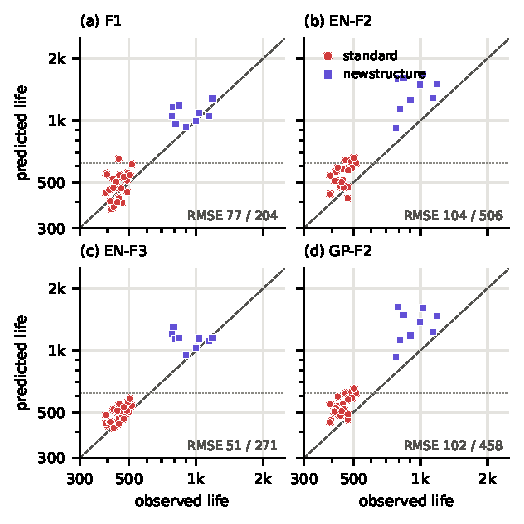
\includegraphics[width=\columnwidth]{fig_rq5_parity}
  \caption{Frozen models on u1 (log axes). RMSE: standard /
  \texttt{newstructure} cells. Dotted: constant baseline (622 cycles).}
  \label{fig:rq5}
\end{figure}

\subsection{Explanation with SHAP}
Exact SHAP values of the predicted $\log_{10}$ life were computed for EN-F2
and EN-F3 with the training cells as background. Fig.~\ref{fig:shap} splits
the mean prediction of each test set into feature contributions and compares
it with the actual mean; the gap is the bias.

\begin{figure}[!htb]
  \centering
  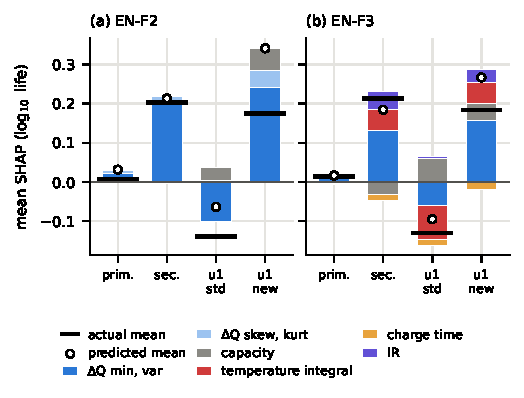
\includegraphics[width=\columnwidth]{fig_rq5_shap}
  \caption{Mean SHAP contribution of each feature group per test set,
  relative to the mean training prediction. Circle: mean prediction; bar:
  actual mean.}
  \label{fig:shap}
\end{figure}

\begin{itemize}
  \item \textbf{EN-F2 over-predicts the standard cells because of their
  capacity.} $\dq$ lowers the prediction ($-0.10$ in $\log_{10}$ life) but
  the high initial capacity raises it ($+0.04$), giving $-0.06$ against an
  actual $-0.14$.
  \item \textbf{EN-F3 is right on the standard cells partly for the wrong
  reason.} Its temperature integral, in effect the long cycle duration,
  lowers the prediction by 0.09 ($\approx-19$\,\%) and cancels the capacity
  effect.
  \item \textbf{The \texttt{newstructure} error comes from $\dq$ itself.}
  The $\dq$ terms add $+0.28$ in EN-F2 against an actual $+0.18$: these cells
  change their discharge curve less than cells of the same life in the other
  batches. No single out-of-range feature is responsible.
\end{itemize}

In EN-F3 the share of the temperature integral rises from 18\,\% of the
attribution on the training cells to 31\,\% on u1, and that of $Q_{d,2}$
from 12 to 23\,\%: the models lean most on the features that lie furthest
outside their training range.

\textbf{Answer to RQ5.} The standard cells, which resemble b2, are
predicted to within 9--14\,\% by EN-F3 and F1; the \texttt{newstructure}
cells are over-predicted by 17--62\,\% by every model because their $\dq$ is
smaller than their life implies. Batch-dependent features help only when the
new batch resembles a training batch, and the simplest model, F1, is the
most robust overall.
